JavaScript was an important addition to the set of web technologies as it is the foundation forweb applications \parencite{ParkJungMoon2015}. Since the introduction, evolution and increased performance of JavaScript, the web has evolved from simply being a platform for websites to also be a platform for web applications \parencite{SandhuHerreraHendren2018}. Web applications, or web apps for short, is a type of application that run inside a web browser. Web apps require no installation and runs on any computing device for which there is a web browser \parencite{RatanaworabhanLivshitsZorn2010}. Figure \ref{google-docs} illustrates Google Docs, a complete wordprocessing application for the web.

\begin{figure}[!h]
\centering
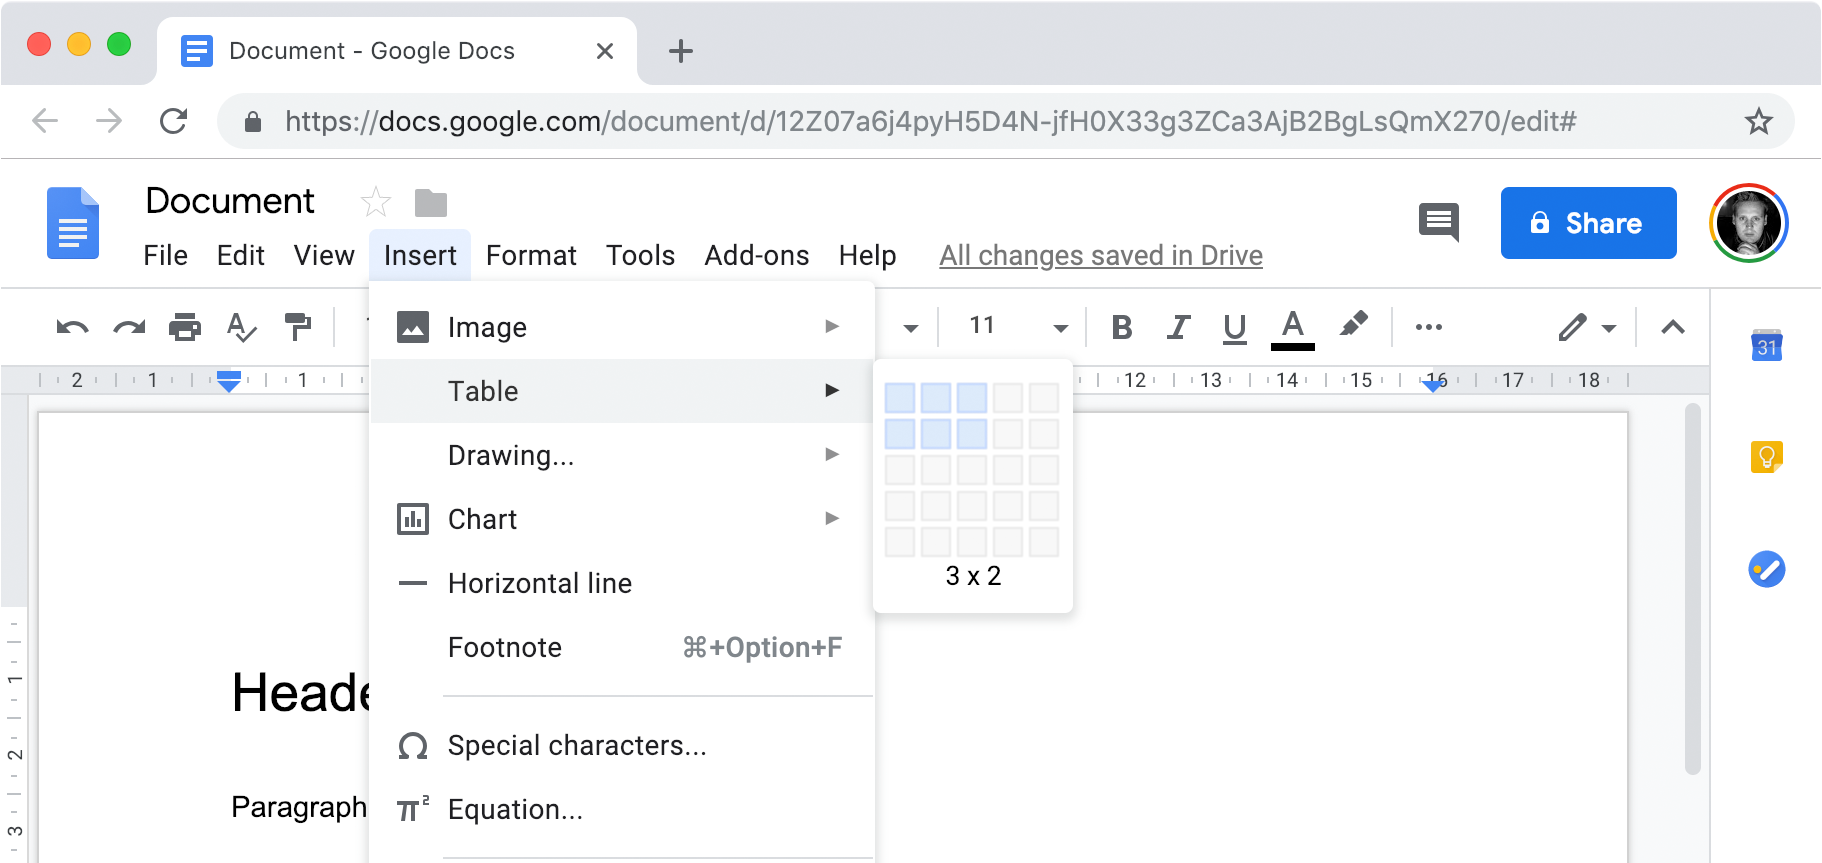
\includegraphics[width=16cm,keepaspectratio]{../Figures/google-docs}
\caption{Google Docs is a modern web application that enables users to do word processing in a web browser.}
\label{google-docs}
\end{figure}

Traditionally web applications was built with a thin user interface layer through which the user interacted with the application, while the actual computation was executed on one or more servers, % in the cloud
passing data back and forth between the client and the server. As modern devices becomes increasingly more powerful, more and more web apps are built to do computing client side.

\textcite{SandhuHerreraHendren2018} describe JavaScript as increasingly popular for building high performance apps and \textcite{RatanaworabhanLivshitsZorn2010} describes the complexity of web apps as the catalyst for browser vendors to increase JavaScript performance. According to \textcite{RatanaworabhanLivshitsZorn2010} the increased usage of sophisticated mobile phones also increasing the importance of web apps.
